\chapter{Conclusions}
\graphicspath{{conclusions/figs}}

A brief introduction

\section{Research Conclusions}
\subsubsection{\nameref{chapter:continuous_compost_bomb}}

In \cref{chapter:continuous_compost_bomb} I investigated the the effect of adding a vertical spatial dimension to the compost bomb instability.
The purpose of this was twofold. 
Firstly, I was interested to see if the instability still existed in a more realistic model.
Secondly, I wanded to know if certain wildfires could be caused by biogeochemical heating and in order to do this more realistic physics was desirable.

\todo[inline]{Expand on Siberian wildfires. add a para?}

In order to investigate this, I created a partial differential equation model of soil temperature which included biogeochemical heating. I made the assumption
that soil carbon could be viewed as being time invariant, which placed the model into the `compost bomb limit' of~\cite{Luke2011}. This came at the cost of preventing
R-tipping so the potential for B-tipping was investigated. Furthermore the effect of a large seasonal cycle in atmospheric temperatures on the soil was investigated.

It was shown that for sufficently large atmospheric temperatures the model had no steady state. This meant that the soil temperatures had diverged and that a compost bomb
had occured. If, as in the real world, soil carbon were allowed to evolve dynamically then the amount of soil carbon would decrease which would prevent the soil temperatures from diverging;
instead they would simply reach a large value.

It was also shown that a sufficently large seasonal cycle --- which could be realised by a summer heat wave --- would be enough to trigger a compost bomb.
Furthermore, the size of the seasonal cycle was not dissimilar to the seasonal cycles observed in parts of Siberia (as shown in \cref{fig:seasonal_cycle_maps}).
This can be seen as evidence that Siberian wildfires may be caused, in part, by biogeochemical heating. 

\begin{figure}
  \centering
  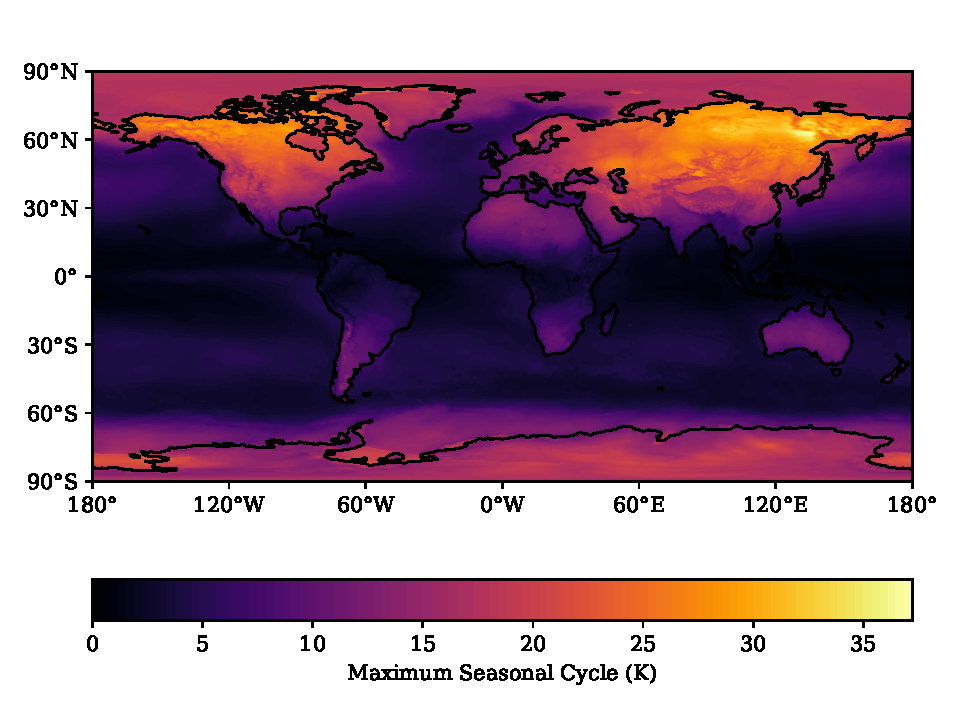
\includegraphics[width=\textwidth,keepaspectratio]{seasonal_cycles}
  \caption[Map of Seasonal Cycles]{The largest observed seaonsonal cycle in the ERA5 reanalysis \parencite{Hersbach2020} over the period 1940--2022.
    The magnitude of the seasonal cycle is defined as half the difference between the maximum and minimum monthy averaged \SI{2.0}{\meter} air temperatures.}
  \label{fig:seasonal_cycle_maps}
\end{figure}

\todo[inline]{misc crit of model}

Due to the approximation that soil carbon was constant in time, the compost bomb instability became an example of B-tipping rather than R-tipping. It does not necessarily
follow that the system would experience R-tipping if this approximation was relaxed. However, it is reasonable to assume that the vertical diffusion of heat would not be a barrier to
R-tipping, as long as the atmospheric temperatures were raised rapidly compared to the soil carbon timescale, due to the significant timescale separation between the soil thermal and
carbon timescales \parencite{Luke2011}.

The approximation that soil carbon is constant is accurate over the timescales of a year, given the decadal turnover time of soil carbon \parencite{Varney2020}.
It follows therefore, that there can be good confidence about the results to do with the seaonal cycle. However, the applicability to the phenomenon of wildfires is more doubtful.
This is because it may be better to view a hot summer period as a more temporally compact perturbation to atmospheric temperatures, rather than an amplified sinusoid. This case has
since been studied by~\cite{OSullivan2023} for the model of~\cite{Luke2011}. They also found for realistic Siberian summer temperatures compost bombs were possible. 

To summarise, in \cref{chapter:continuous_compost_bomb} I managed to show that adding in the vertical diffusion of heat does not suppress the compost bomb. This therefore increases the confidence
that the effect is real. Furthermore I also showed that a hot summer, as modeled by a large seasonal cycle of temperature, could cause compost bombs, which has applications to the
problem of Siberian wildfires.

\subsubsection{\nameref*{chapter:global_bomb}}

The investigation into the role of biogeochemical heating was continued in \cref{chapter:global_bomb}. Instead of looking at the local effect of biogeochemical heating,
the effect at the global scale was considered. This was motivated by the fact that the extra carbon released by biogeochemical heating would increase atmospheric temperatures,
further increasing respiration. This positive feedback therefore increases the chances of triggereing a compost bomb, and it is thus important to quantify.\todo{I can write this better}

In order to do this, the model of~\cite{Luke2011} was assumed to hold at the global scale, meaning quanitites could be replaced with their globally averaged values. The air temperature
was set to scale logarithmically with atmospheric \ce{CO2}, which in turn was calculated through carbon conservation. The additional effect of \ce{CO2} fertilisation was considered,
by assuming Net Primary Productivity was a saturating function of atmospheric carbon. The role of the ocean was accounting for very simply, by assuming that a fixed fraction of
carbon emissions become ocean carbon, which is equivalent to scaling down the flux from the land to the atmosphere by a fixed amount.

The stability of this model was investigated first. To do this its bifurcation diagram was computed and it was found that there was a bifurcation if the climate sensitivity was large enough
or the biogeochemical heating was strong enough. The model was simple enough that the location of the bifurcation point could be computed analytically. The effect of linearly increasing
atmospheric carbon was then investigated, where it was shown numerically that R-tipping could occur and contribution to atmospheric \ce{CO2} from biogeochemical heating was quantified.

It was found that for realistic amounts of biogeochemical heating, only a small difference to the stability of the system was made. It was however striking, that when there was no
\ce{CO2} fertilisation, the system was unstable at comparatively low levels of climate sensitivity. These levels are low enough to be in the range of CMIP models. It is therefore interesting to note
that without \ce{CO2} fertilisation the Earth's carbon and thus climate system may not be stable.

The critical rates of emissions required to trigger a compost bomb in this system was also determined. It was found that these critical rates far exceeded anything humanity was likely to be able
to emit. Furthermore contribution to atmospheric \ce{CO2} was found to be small. It was however interesting to note that \ce{CO2} decreased these critical rates and increased the impact of
biogeochemical heating on carbon emissions to the atmosphere. Furthermore, it was found that there was an `optimal' climate sensitivity which maximised the impact of biogeochemical heating
on carbon emissions at that this optimum occured at plausible values of the climate sensitivity.

This approach to analysing the role of biogeochemical heating has its problems. To begin with, as demonstrated in \cref{chapter:continuous_compost_bomb}, biogeochemical heating
can be important regionally, yet this global modelling approach greatly reduces its influence. For example, for some combination of climate sensitivity and biogeochemical heating
it could be the case that a region of the Earth has an unstable carbon cycle whereas the global analysis would give a stable carbon cycle. This is problematic as an instability in one
region of the Earth could propogate to give a global instability. A similar logic applies to the determination of the critical rates and the contribution to atmospheric \ce{CO2}.
This would therefore imply that the analysis in \cref{chapter:global_bomb} overestimates the stability of the carbon cycle and underestimates the critical rates and contribution to atmospheric
\ce{CO2}.

Other modelling assumptions are also suspect. For example, it was assumed that atmospheric temperatures adjust instantaneously to increases in atmospheric \ce{CO2}, but in
reality this process can take years \parencite{Rugenstein2019}. It was also assumed that the ocean could be modelled as absorbing a fixed fraction of carbon, an assumption that is serverly questioned in
\cref{chapter:conceptual_carbon_cycle}.

\Cref{chapter:global_bomb} set out to analyse the effect, at the global scale, of biogeochemical heating. Due to the problems caused by biogeochemical heating
being so regionally heterogeneous, firm conclusions cannot be drawn. However, more confidence can be had in the role \ce{CO2} fertilisation and climate-carbon
sensitivity play. \ce{CO2} fertilisation acts to destabalise the system with respect to biogeochemical heating, although it still plays a stabalising role
overall. The terrestrial carbon system is most unstable at higher values of the climate-carbon sensitivity but a lower value of this sensitivity does not
necessarily imply a smaller flux of carbon to the atmosphere due to biogeochemical heating.

\subsubsection{\nameref*{chapter:conceptual_carbon_cycle}}

In \cref{chapter:global_bomb}, it was noted that the Earth's terrestrial carbon cycle was stable for only some values of the climate-carbon sensitivity and that at low
\ce{CO2} fertilisation this critical sensitivity was very low. \Cref{chapter:conceptual_carbon_cycle} took these ideas further to investigate which parameter combinations
were compatible with the reconstructed behaviour of atmospheric \ce{CO2} in the the pre-industrial Holocene epoch. During this epoch, \ce{CO2} showed little variability
and appeared be following a slowly changing equilibrium. \todo{How much variability?}

In order to constrain the parameters a better ocean model was required than was used in \cref{chapter:global_bomb}. In \cref{chapter:conceptual_carbon_cycle}
the ocean carbon cycle from the IMOGEN model was used in addition to simplified box models. Biogeochemical heating was also not accounted for on the grounds
that \cref{chapter:global_bomb} had found the effect weak at the global scale.

Using the IMOGEN ocean carbon cycle model, it was found that there was a critical value of cliamte sensitivity beyond which the carbon cycle would become unstable.
The bifurcation appeared to be a Hopf bifurcation. The oscillations after the bifurcation had a large amplitude and are incompatible with the observed bahviour of the
carbon cycle.

Using a two box model, these results could be recreated. Furthermore, that the bifurcation was a Hopf bifurcation could be confirmed and the bifurcation point
could analytically be determined. The two box model could give a Hopf bifurcation at the same point in parameter space as the IMOGEN model.

A one box model was also formulated, which could show a bifurcation of various types depending on the choice of the timescale of the box.
For a fast timescale, this was a transcritical bifurcation, similar to the system analysed in \cref{chapter:global_bomb}. Furthermore, because the bifurcation
point could be analytically computed, this can be compared to the bifurcation point derived in \cref{chapter:global_bomb} to give an interpretation to the
ocean model in that chapter. It was found that the ocean model in \cref{chapter:global_bomb} was self-consistent only when the ocean timescale was very short.
If the timescales were longer, the bifurcation was a Hopf bifurcation, however the bifurcation point was at a different point in parameter space to that of IMOGEN.

The critical climate sensitivities found using the IMOGEN model were, for realistic values of \ce{CO2} fertilisation, around \SI{10}{\kelvin} which could be
related to equilibrium climate sensitivities around \SI{6}{\kelvin}. These values are not significantly larger than those found in CMIP6 \parencite{Zelinka2020}.
This raises the possibility that when performing coupled climate-carbon simulation some of these models may not be able to simulate a stable pre-industrial
period. Furthermore those models which have low enough climate sensitivity to not cross the bifurcation may still have unrealistic levels of \ce{CO2} variability
due to the phenomenon of critical slowing down. As climate models increase the complexity of their carbon cycle representations by including, for example,
nutrient limitation, the magnitude of the \ce{CO2} fertilisation effect may decrease \parencite{Wiltshire2021}, which would make these models more likely to be unstable.

The analysis in \cref{chapter:conceptual_carbon_cycle} ignored certain effects. It ignored the climate effect on net primary producticity, which is likely to weaken
net primary productivity in the tropics and strengthen it in the high latitudes \todo{Cite this}.
However, this effect is small relative to the effect of \ce{CO2} fertilisation \parencite{Arora2020}.
It also made the same assumptions about the instantaneous temperature equilibration to atmospheric \ce{CO2} as did \cref{chapter:global_bomb}.
Whilst this may effect the behaviour of the carbon cycle beyond the bifurcation when \ce{CO2} is changing;
it is unlikely to effect the position of the bifurcation much as the system as \ce{CO2} levels are constant before the bifurcation and thus the equilibrium assumption is more reasonable.

In summary, \cref{chapter:conceptual_carbon_cycle} showed that certain parameter regemes were not compatible with the behaviour of \ce{CO2} over the Holocene.
This behaviour could be recreated using a two box model, suggesting the importance of two timescales. Furthermore the critical parameter values identified are close to those in
some CMIP6 models suggesting that they would not be able to give a stable Holocene if run in a coupled climate-carbon configuration.

\subsubsection{\nameref*{chapter:spatial_ews}}

\subsubsection{\nameref*{chapter:rosa}}

\subsubsection{Synthesis}

\section{Outlook}

A graceful landing?